\documentclass{article}

  % packages
    % basic stuff for rendering math
    \usepackage[letterpaper, top=1in, bottom=1in, left=1in, right=1in]{geometry}
    \usepackage[utf8]{inputenc}
    \usepackage[english]{babel}
    \usepackage{amsmath} 
    \usepackage{amssymb}
    \usepackage{bookmark}

    % extra math symbols and utilities
    \usepackage{mathtools}        % for extra stuff like \coloneqq
    \usepackage{mathrsfs}         % for extra stuff like \mathsrc{}
    \usepackage{centernot}        % for the centernot arrow 
    \usepackage{bm}               % for better boldsymbol/mathbf 
    \usepackage{enumitem}         % better control over enumerate, itemize
    \usepackage{hyperref}         % for hypertext linking
    \usepackage{xr-hyper}
    \usepackage{fancyvrb}          % for better verbatim environments
    \usepackage{newverbs}         % for texttt{}
    \usepackage{xcolor}           % for colored text 
    \usepackage{listings}         % to include code
    \usepackage{lstautogobble}    % helper package for code
    \usepackage{parcolumns}       % for side by side columns for two column code
    \usepackage{algorithm}
    \usepackage{algpseudocode}
    \usepackage{bbm}
    \algblock{Class}{EndClass}

    % page layout
    \usepackage{fancyhdr}         % for headers and footers 
    \usepackage{uniquecounter}
    \usepackage{lastpage}         % to include last page number in footer 
    \usepackage{parskip}          % for no indentation and space between paragraphs   
    \usepackage[T1]{fontenc}      % to include \textbackslash
    \usepackage{footnote}
    \usepackage{etoolbox}

    % for custom environments
    \usepackage{tcolorbox}        % for better colored boxes in custom environments
    \tcbuselibrary{breakable}     % to allow tcolorboxes to break across pages

    % figures
    \usepackage{pgfplots}
    \pgfplotsset{compat=1.18}
    \usepackage{float}            % for [H] figure placement
    \usepackage{tikz}
    \usepackage{tikz-cd}
    \usepackage{circuitikz}
    \usetikzlibrary{arrows, arrows.meta}
    \usetikzlibrary{positioning}
    \usetikzlibrary{calc}
    \usepackage{graphicx}
    \usepackage{caption} 
    \usepackage{subcaption}
    \captionsetup{font=small} 

    % for tabular stuff 
    \usepackage{dcolumn}

    \usepackage[nottoc]{tocbibind}
    \pdfsuppresswarningpagegroup=1
    \hfuzz=5.002pt                % ignore overfull hbox badness warnings below this limit

  % New and replaced operators
    \DeclareMathOperator{\Tr}{Tr}
    \DeclareMathOperator{\Sym}{Sym}
    \DeclareMathOperator{\Span}{span}
    \DeclareMathOperator{\elbo}{ELBO}
    \DeclareMathOperator{\std}{std}
    \DeclareMathOperator{\Cov}{Cov}
    \DeclareMathOperator{\Var}{Var}
    \DeclareMathOperator{\Corr}{Corr}
    \DeclareMathOperator{\pos}{pos}
    \DeclareMathOperator*{\argmin}{\arg\!\min}
    \DeclareMathOperator*{\argmax}{\arg\!\max}
    \newcommand{\qed}{\hfill$\blacksquare$}     % I like QED squares to be black

  % Custom Environments
    \newtcolorbox[auto counter, number within=section]{question}[1][]
    {
      colframe = orange!25,
      colback  = orange!10,
      coltitle = orange!20!black,  
      breakable, 
      title = \textbf{Question \thetcbcounter ~(#1)}
    }

    \newtcolorbox[auto counter, number within=section]{exercise}[1][]
    {
      colframe = teal!25,
      colback  = teal!10,
      coltitle = teal!20!black,  
      breakable, 
      title = \textbf{Exercise \thetcbcounter ~(#1)}
    }
    \newtcolorbox[auto counter, number within=section]{solution}[1][]
    {
      colframe = violet!25,
      colback  = violet!10,
      coltitle = violet!20!black,  
      breakable, 
      title = \textbf{Solution \thetcbcounter}
    }
    \newtcolorbox[auto counter, number within=section]{lemma}[1][]
    {
      colframe = red!25,
      colback  = red!10,
      coltitle = red!20!black,  
      breakable, 
      title = \textbf{Lemma \thetcbcounter ~(#1)}
    }
    \newtcolorbox[auto counter, number within=section]{theorem}[1][]
    {
      colframe = red!25,
      colback  = red!10,
      coltitle = red!20!black,  
      breakable, 
      title = \textbf{Theorem \thetcbcounter ~(#1)}
    } 
    \newtcolorbox[auto counter, number within=section]{corollary}[1][]
    {
      colframe = red!25,
      colback  = red!10,
      coltitle = red!20!black,  
      breakable, 
      title = \textbf{Corollary \thetcbcounter ~(#1)}
    } 
    \newtcolorbox[auto counter, number within=section]{proof}[1][]
    {
      colframe = orange!25,
      colback  = orange!10,
      coltitle = orange!20!black,  
      breakable, 
      title = \textbf{Proof. }
    } 
    \newtcolorbox[auto counter, number within=section]{definition}[1][]
    {
      colframe = yellow!25,
      colback  = yellow!10,
      coltitle = yellow!20!black,  
      breakable, 
      title = \textbf{Definition \thetcbcounter ~(#1)}
    } 
    \newtcolorbox[auto counter, number within=section]{example}[1][]
    {
      colframe = blue!25,
      colback  = blue!10,
      coltitle = blue!20!black,  
      breakable, 
      title = \textbf{Example \thetcbcounter ~(#1)}
    } 
    \newtcolorbox[auto counter, number within=section]{code}[1][]
    {
      colframe = green!25,
      colback  = green!10,
      coltitle = green!20!black,  
      breakable, 
      title = \textbf{Code \thetcbcounter ~(#1)}
    } 
    \newtcolorbox[auto counter, number within=section]{algo}[1][]
    {
      colframe = green!25,
      colback  = green!10,
      coltitle = green!20!black,  
      breakable, 
      title = \textbf{Algorithm \thetcbcounter ~(#1)}
    } 
    \definecolor{cverbbg}{gray}{0.93}
    \newenvironment{cverbatim}
      {\SaveVerbatim{cverb}}
      {\endSaveVerbatim
        \flushleft\fboxrule=0pt\fboxsep=.5em
        \colorbox{cverbbg}{%
          \makebox[\dimexpr\linewidth-2\fboxsep][l]{\BUseVerbatim{cverb}}%
        }
        \endflushleft
    }

    \definecolor{dkgreen}{rgb}{0,0.6,0}
    \definecolor{gray}{rgb}{0.5,0.5,0.5}
    \definecolor{mauve}{rgb}{0.58,0,0.82}
    \definecolor{lightgray}{gray}{0.93}
    \renewcommand{\algorithmiccomment}[1]{\hfill$\triangleright$\textcolor{blue}{#1}}

    % default options for listings (for code)
    \lstset{
      autogobble,
      frame=ltbr,
      language=Python,                           % the language of the code
      aboveskip=3mm,
      belowskip=3mm,
      showstringspaces=false,
      columns=fullflexible,
      keepspaces=true,
      basicstyle={\small\ttfamily},
      numbers=left,
      firstnumber=1,                        % start line number at 1
      numberstyle=\tiny\color{gray},
      keywordstyle=\color{blue},
      commentstyle=\color{dkgreen},
      stringstyle=\color{mauve},
      backgroundcolor=\color{lightgray}, 
      breaklines=true,                      % break lines
      breakatwhitespace=true,
      tabsize=3, 
      xleftmargin=2em, 
      framexleftmargin=1.5em, 
      stepnumber=1
    }

  % Page style
    \pagestyle{fancy}
    \fancyhead[L]{Attention Models}
    \fancyhead[C]{Muchang Bahng}
    \fancyhead[R]{Spring 2023} 
    \fancyfoot[C]{\thepage / \pageref{LastPage}}
    \renewcommand{\footrulewidth}{0.4pt}          % the footer line should be 0.4pt wide
    \renewcommand{\thispagestyle}[1]{}  % needed to include headers in title page
%    \renewcommand{\thefootnote}{\arabic{footnote}}

  % external documents 
    \externaldocument[algo-]{../../Computer_Science/DSA/paper}[../../Computer_Science/DSA/paper.pdf]

\begin{document}

\tikzset{every picture/.style={line width=0.75pt}} 

\title{Attention-Based Models}
\author{Muchang Bahng}
\date{Spring 2023}

\maketitle
\tableofcontents
\pagebreak 


This covers computability theory, complexity theory, and automata theory. 
Alphabet. Boolean logic



\section{Attention Models}

  We have seen the power of encoder decoder models, which can be used with a combination of RNNs or CNNs. Since we can plug and play different architectures, we can process and output different types of data.\footnote{CNNs can be used to encode or output images and RNNs can be used to encode or output sequential data.} CNNs were quite strong and have really no problem with scaling ever since the ResNet architecture, but historically, RNNs had two main problems. 
  \begin{enumerate} 
    \item They compute sequentially, since the hidden states must be a function of previous hidden states. This results in a linear time complexity, which is not ideal. 
    \item By encoding the entire sequence in a hidden latent space of dimension $h$, we are essentially trying to compress a possibly very long sequence into a single vector of predetermined dimension. This causes a \textit{bottleneck problem} and words that are further away may be ``forgotten.''
  \end{enumerate}

  We will see that attention solves the second bottleneck problem, and self-attention solves the sequential problem. 

  In general, feed forward networks treat features as independent, convolutional networks focus on relative location and proximity, and RNNs have tend to read in one direction. This may not be the most flexible way to process data, and we have some other problems. 
  \begin{enumerate}
      \item When processing images, we may want our CNN to focus on a specific part of the image. For example, when we see a cat in the corner, other parts of the image does not matter, and we can have our CNN focus on the specific portion of the image containing the cat. 
      \item When reading sentences, different words may be interdependent, even if they are not next to each other, and so we may want to focus on different portions of a sentence (e.g. words 1~3, plus 10~15 which describes an object). 
  \end{enumerate}

  This is where attention comes in to the rescue. Attention is, to some extent, motivated by how we pay visual attention to different regions of an image or correlate words in one sentence. Human attention allows us to focus on certain regions or portions of our data with ``high resolution" while perceiving the surrounding data in ``low resolution." In a nutshell, attention in deep learning can be broadly interpreted as a vector of importance weights. First, we will introduce attention in the general setting, then move onto its specific implementation in RNNs through the seq2seq attention model, and finally its application in CNNs through Vision transformers. 

\subsection{Seq2Seq with Attention}

  The idea of \textbf{attention} provides a solution to this bottleneck problem. Basically, we want to establish connections from the decoder to not just the last hidden state of the encoder, but to all of its nodes. Each encoder node represents some information about each word, and by taking some weighted sum of these nodes, we can choose which one to put this attention on. 

  \begin{definition}[Score Function]
    Before we begin, let's define a metric, called a \textbf{score function}, to determine how similar two words (more specifically, their embeddings) are. The two simplest ways to do this are: 
    \begin{enumerate}
      \item the standard dot product. 
        \begin{equation}
          \mathrm{score}(\mathbf{x}, \mathbf{y}) = \mathbf{x} \cdot \mathbf{y} 
        \end{equation}
      \item cosine similarity. 
        \begin{equation}
          \mathrm{score}(\mathbf{x}, \mathbf{y}) = \frac{\mathbf{x} \cdot \mathbf{y}}{||\mathbf{x}|| \, ||\mathbf{y}||}
        \end{equation}
    \end{enumerate}
  \end{definition}

  Now that we have the score defined, the heart of attention comes with the query, key, value model. The general idea is this: for every prediction we want to make (whether it is classifying something or generating a new output word/token), we want to get its respective query vector and use it to look through key-value dictionary in order to get the most relevant information from it. With this information, combined with the query and whatever other information we have, we can make a prediction. 

  Let's go through this step by step. What we want to do is associate every input hidden node $\mathbf{h}_t$ with a 2-tuple consisting of a key-value pair. 

  \begin{equation}
    \mathbf{h}_t \mapsto (\mathbf{k}_t, \mathbf{v}_t)
  \end{equation}

  and associate every hidden output node $\mathbf{s}_t$ with a query value. 
  \begin{equation}
    \mathbf{s}_T \mapsto \mathbf{q}_t
  \end{equation}

  \begin{definition}[Seq2Seq with Vanilla Attention] 
    Eventually, we would like to learn these key, value, queries, but for now let's focus on the forward propagation. 
    \begin{enumerate}
      \item The input has been sequentially encoded and we have a special start token $\mathbf{s}_0$. 
      \item For $t^\prime = 0$ until the $\mathbf{s}_{T^\prime}$ is the end token, do the following. 
      \begin{enumerate}
        \item Take the query $\mathbf{s}_i$ and compute the attention score $\mathrm{score}(\mathbf{s}_i, \mathbf{h}_t)$ for all $t = 1, \ldots, T$. This determines which encoder hidden state we should pay attention to. 
        \begin{equation}
          \mathbf{e}^{t^\prime} = \big[ \mathrm{score}(\mathbf{s}_{t^\prime}, \mathbf{h}_1 ), \ldots, \mathrm{score}(\mathbf{s}_{t^\prime}, \mathbf{h}_T) \big] \in \mathbb{R}^T
        \end{equation}

        \item We take its softmax to get the \textbf{attention distribution} $\boldsymbol{\alpha}^{t^\prime}$ for this step (a discrete probability distribution) 
        \begin{equation}
          \boldsymbol{\alpha}^{t^\prime} = \mathrm{softmax} (\mathbf{e}^{t^\prime}) \in \mathbb{R}^T
        \end{equation}

        \item We use $\boldsymbol{\alpha}^{t^\prime}$ to take a weighted sum of the encoder hidden states to get the attention output $\mathbf{a}_t$ 
        \begin{equation}
          \mathbf{a}_{t^\prime} = \sum_{t=1}^T \alpha_{t}^{t^\prime} \mathbf{h}_t \in \mathbb{R}^h
        \end{equation}
        which acts as our context vector $\mathbf{C}_{t^\prime}$ that we can now use in our vanilla seq2seq model.\footnote{This weighted sum is a selective summary of the information contained in the values, where the query determines which values to focus on. Attention is a way to obtain a fixed size representation of an arbitrary set of representations (the values), dependent on some other representation (the query).} Note that this context vector is different for every $\mathbf{s}_{t^\prime}$, so at every step we can choose which encoder states/words to focus on. \footnote{This is similar to a hash map where you have a set of key-value pairs. When you have a query, you want to search through the keys to see if it matches the query, and then it returns the value of the matched key. In our case, we have a query, and rather than looking for exact matches, we want to return a similarity score of the query $q_i$ across all $k_i$'s and provide a weighted sum of the corresponding values.} 
      \end{enumerate}
    \end{enumerate}

    Another trick to improve performance is that these attention context vectors can be concatenated with the previous decoder hidden state to get more information in the already decoded part of the sentence.   

    \begin{center}
      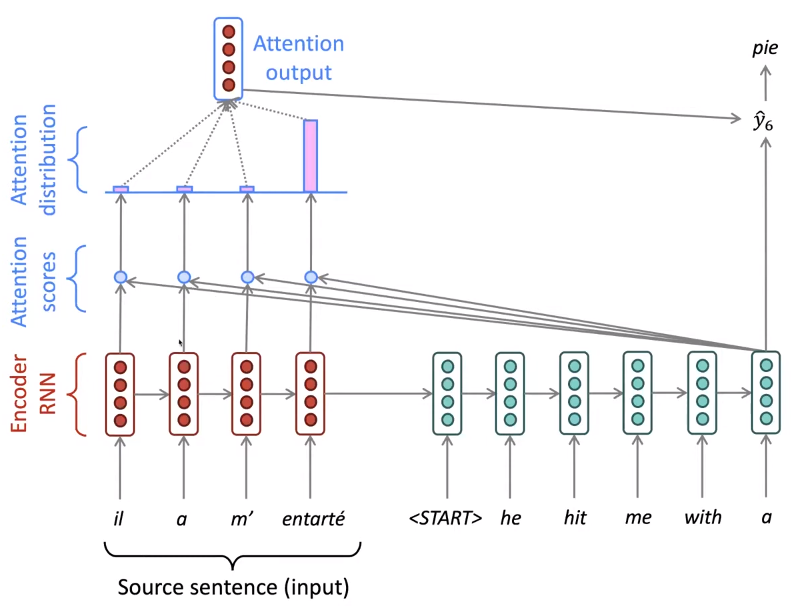
\includegraphics[scale=0.4]{img/seq2seq_attention.png}
    \end{center}
  \end{definition}

  Overall, attention is extremely useful in improving all performance, and it is intuitive with how humans analyze things, too. It significantly improves neural machine translation by allowing the decoder to focus on certain parts of the source. It also provides more ``human-like" model of the machine translation process (you can look back at the source sentence while translating, rather than needing to remember it all). It solves the bottleneck problem and helps with the vanishing gradient problem with these pseudo-residual connections through the context vector. 

  Finally, it provides some interpretability, as we can inspect the attention distribution to see what the decoder was focusing on (which again, we've never set explicitly but was learned by the model). 

  \begin{center}
    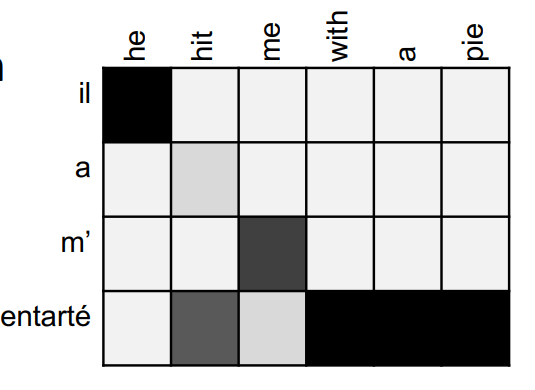
\includegraphics[scale=0.3]{img/attention_distribution.png}
  \end{center}

  \begin{code}
    For an implementation of this in PyTorch, look \href{code/seq2seq_attention.ipynb}{here}.
  \end{code}

  Now let's talk about how these parameters are already learned. The parameters of the model are. 
  \begin{enumerate}
    \item The encoding matrices for the usual seq2seq model: $\mathbf{W}_e, \mathbf{U}_e$. 
    \item Generating key, value, and query vectors for every possible embedding is not practical.\footnote{You would need three $d_{\mathrm{embedding}} \times |\mathcal{V}|$ matrices, where $\mathcal{V}$ is the set of our vocabulary, which can go easily past 500,000 elements.} A more compact way to represent them are through linear maps, so we are learning matrices $\mathbf{Q}, \mathbf{K}, \mathbf{V}$ such that 
    \begin{align*}
      \mathbf{q}_{t^\prime} & = \mathbf{Q} \mathbf{s}_{t^\prime} \\ 
      \mathbf{k}_t & = \mathbf{K} \mathbf{h}_t \\
      \mathbf{v}_t & = \mathbf{V} \mathbf{h}_t
    \end{align*}

    \item We should now have the decoding matrices $\mathbf{W}_d$ that takes in the attention context vector (plus maybe the previous hidden decoder state) and the original matrix $\mathbf{U}_d$. 
  \end{enumerate}
  Therefore, this problem reduces to learning the matrices $\mathbf{W}_e, \mathbf{U}_e, \mathbf{Q}, \mathbf{K}, \mathbf{V}, \mathbf{W}_d, \mathbf{U}_d$. 

  \begin{example}[Score Functions]
    Having additional flexibility with the score functions can also improve learning. We provide more examples here, which give more parameters to learn as well.  
    \begin{enumerate}
      \item The general attention model allows us to train a shared-weight matrix, allowing for $s \neq h$. 
      \[e^{t^\prime}_t = \mathrm{score}(\mathbf{s}_{t^\prime}, \mathbf{h}_t) = \mathbf{s}_{t^\prime}^T \mathbf{W}_a \mathbf{h}_t \in \mathbb{R}\]
      However, it may seem like there are too many parameters in $\mathbf{W}_a$, having to learn $sh$ values. 

      \item The reduced rank multiplicative attention uses low rank matrices, allowing us to learn only $ks + kh$ parameters for matrices $\mathbf{U}_a \in \mathbb{R}^{k \times s}, \mathbf{V}_a \in \mathbb{R}^{k \times h}$ where $k << s, h$. 
      \[e^{t^\prime}_t = \mathrm{score}(\mathbf{s}_{t^\prime}, \mathbf{h}_t) = \mathbf{s}_{t^\prime}^T (\mathbf{U}_a^T \mathbf{V}_a) \mathbf{h}_t = (\mathbf{U}_a \mathbf{s}_{t^\prime})^T (\mathbf{V}_a \mathbf{h}_t) \in \mathbb{R}\]

      \item Additive attention uses a neural net layer defined 
      \[e^{t^\prime}_t = \mathbf{v}_a^T \mathrm{tanh}(\mathbf{W}_a \mathbf{h}_t + \mathbf{V}_a \mathbf{s}_{t^\prime}) \in \mathbb{R}\]
      where $\mathbf{W}_a \in \mathbb{R}^{r \times h}, \mathbf{V}_a \in \mathbb{R}^{r \times s}$ are weight matrices, $\mathbf{v}_a \in \mathbb{R}^r$ is a weight vector, and $r$ (the attention dimensionality) is a hyperparameter. 
    \end{enumerate}
  \end{example}

  This can be naturally extended to other architectures, as we will explore later. 

  \begin{example}[Images]
    Given an image of size $224 \times 224$, we can make patches of size $16 \times 16$, and then flatten them to get a $196 \times 768$ matrix with a 2-dimensional positional encoding scheme. We can then apply a linear transformation to get the query, key, and value vectors.
  \end{example}

\subsection{Self-Attention Layer}

    While we have solved the bottleneck problem, this entire process is still sequential since every hidden decoder node requires us to know the previous hidden node. There are two sequential processes in the regular seq2seq attention model. 
    \begin{enumerate}
      \item The sequential encoding of the input sentence. 
      \item The sequential decoding of the output sentence. This unfortunately is not possible in transformers to parallelize. 
    \end{enumerate}

    We will focus on parallelizing the first part by temporarily forgetting about encoder-decoder models and just thinking about how to incorporate a good encoder with attention that is parallelizable \cite{vaswani2017attention}. This extension is quite simple. Let $\mathbf{w}_{1:n}$ be a sequence of words in vocabulary $\mathcal{V}$. The key here is that rather than inputs having key-values and outputs having queries, \textit{all} words are associated with a 3-tuple of key, value, query. 
    \begin{equation}
      \mathbf{x}_i \mapsto (\mathbf{q}_i, \mathbf{k}_i, \mathbf{v}_i)
    \end{equation}

    \begin{definition}[Standard Scaled Dot-Product Attention]
      If we keep the score function to be the dot-product, the derivations become quite simple. 
      \begin{enumerate}
        \item For each $\mathbf{w}_i$, let $\mathbf{x}_i = E \mathbf{w}_i$ be the word embedding (with $E \in \mathbb{R}^{d \times |\mathcal{V}|}$ the embedding matrix). 

        \item We transform each word embedding with the (learned) weight matrices $\mathbf{Q}, \mathbf{K}, \mathbf{V}$. 
        \begin{align*} 
          \mathbf{q}_i & = \mathbf{Q} \mathbf{x}_i \implies Q = \mathbf{Q} X \\
          \mathbf{k}_i & = \mathbf{K} \mathbf{x}_i \implies K = \mathbf{K} X \\
          \mathbf{v}_i & = \mathbf{V} \mathbf{x}_i \implies V = \mathbf{V} X 
        \end{align*}
        where $X = [x_1, \ldots, x_n] \in \mathbb{R}^{d \times n}$.  

        \item We compute pairwise similarities between keys and queries and normalize with the softmax to get the attention distribution for each word. 
          \begin{equation}
            \mathbf{e}_{ij} = \mathbf{q}_i^T \mathbf{k}_j , \;\;\; \boldsymbol{\alpha}_{ij} = \frac{\exp(\mathbf{e}_{ij})}{\sum_{j^\prime} \exp(\mathbf{e}_{i j^\prime})}
          \end{equation}

        \item Compute the output for each word as a weighted sum of values. 
          \begin{equation}
            \mathbf{o}_i = \sum_j \boldsymbol{\alpha}_{ij} \mathbf{v}_j 
          \end{equation}
      \end{enumerate}

      Ultimately, this can be parallelized into one matrix operation.\footnote{Note that in order to even do such a thing, we must know $n$ beforehand. This can be solved by simply fixing some maximum length, padding everything to be some null token after the end token, and masking all the null tokens to be $0$. More on masking later. } 

      \begin{equation} 
        \mathrm{Attention}(Q, K, V) = \mathrm{softmax} \bigg( \frac{Q K^T}{\sqrt{E_k}} \bigg) V
      \end{equation}

      where the softmax is done to each row.\footnote{We divide by $\sqrt{E_k}$ to stabilize the gradients since as dimensionality increases, the dot product between random vectors tend to get large, leading to large softmax inputs. You can simply compute the variance of two $d$-dimensional Gaussian vectors and see that their variances scales linearly with $d$. }\footnote{You can see that if we have simple dot-product similarity scores, then $E_k = E_v$, but this need not be true in general. We will explore other similiarity score in the next subsection. } 

      Therefore, when you do a forward pass on an attention layer with input $x$, you first get the query vector $q$, extract the attention-weighted values from the key-value dictionary, and then return the weighted sum of the values. To give explicit parameterizations using the query, key, value encoding matrices, we can write this as 
      \begin{equation} 
        \mathrm{Attention}(x \,;\, \mathrm{Q}, \mathrm{K}, \mathrm{V}) = \mathrm{softmax} \bigg( \frac{(\mathbf{Q}x)(\mathbf{K} x)^T}{\sqrt{E_k}} \bigg) (\mathbf{V} x)
      \end{equation}

      This will give us a vector $\mathbf{o}_{1:n}$ consisting of the encoded vectors for each word in the sentence, and best of all, this is parallelizable! 
    \end{definition}

    There are three problems however. 
    \begin{enumerate}
      \item This self-attention encoding does not account for the position/order of the words. Therefore, some positional embedding is needed. 
      \item Our plan is to stack this layer multiple times on top of each other. However, we are just composing linear maps ultimately, so some nonlinearity is needed. 
      \item To use self-attention in \textit{decoders}, as we will see later on, we don't want to have any attention on later parts of a sentence, so we need some way to \textit{mask} future words. 
    \end{enumerate}

    We will deal with the first two problems and address the third problem in the transformer archictecture. 

  \subsubsection{Tokenization and Positional Embeddings}

    Given an input (or an output) $\mathbf{x}$, it must be tokenized into a sequence of tokens. This is a general preprocessing step that is done for any input, whether it be a sequence of words, a sequence of regions in an image, or a sequence of anything. The raw token data will be denoted $w_i$ for $i = 1, \ldots, n$.We can then embed these tokens into a vector space $x_i \in \mathbb{R}^d$. 

    As we will see later, attention does not have a way to discern the order of the input sequences. Therefore, we must add this positional information to the encoding. The most obvious way would be to simply concatenate the position of the token to the end with an index. 
    \begin{equation} 
      x_i \mapsto [x_i, i]
    \end{equation}
    However, this is not ideal since this tends to corrupt the embedding of the token. Instead, we can think of adding certain vectors representing components to the original embedding. 
    \begin{equation} 
      x_i \mapsto x_i + p_i
    \end{equation}
    Certain ways come to mind, such as simply letting $p_i$ be the vector of all $i$'s. This tends not to work in progress since the values of $i$ get too large and corrupts the embeddings too much.\footnote{A helpful Medium article \href{https://medium.com/@waelrashwan/demystifying-transformer-architecture-the-magic-of-positional-encoding-5fe8154d4a64}{here}} Normalizing the values of $i$ to be in $[0, 1]$ is disadvantageous because now the positional embedding $p_i$ is dependent on the length of the total input sequence. Therefore, we need two properties: 
    \begin{enumerate} 
      \item The positional encoding should be independent of the input sequence length. 
      \item The positional encoding shouldn't be too large that it corrupts the semantic meaning behind the original embedding. 
    \end{enumerate}
    It turns out that the sinusoidal function satisfies these properties. 

    \begin{definition}[Sinusoidal Position Embedding]
      Given the embeddings $x_i \in \mathbb{R}^{d}$, we can add a positional encoding to it by 
      \[x_i \mapsto x_i + p_i\]
      where the positional encoding is given by the vector where each component is defined as 
      \begin{equation} 
        (p_i)_j =  \begin{cases} 
            \sin \big( \frac{i}{10000^{2j/d}} \big) & \text{ if } j \text{ is even} \\ 
            \cos \big( \frac{i}{10000^{2j/d}} \big) & \text{ if } j \text{ is odd}
        \end{cases}
      \end{equation}
      where $i$ iterates through the tokens and $j$ iterates through the dimensions of the embedding. 
    \end{definition}

  \subsubsection{Stacked Attention Layers and Multi-Head Attention}

    The second problem of introducing nonlinearities is quite simple. Once we have the output of the first self-attention layer $\mathbf{o}_{1:n} = [\mathbf{o}_1, \ldots, \mathbf{o}_n]$, we can just input each $\mathbf{o}_i$ through a small MLP to introduce nonlinearity before inputting it into the next self-attention layer. 

    \begin{center}
      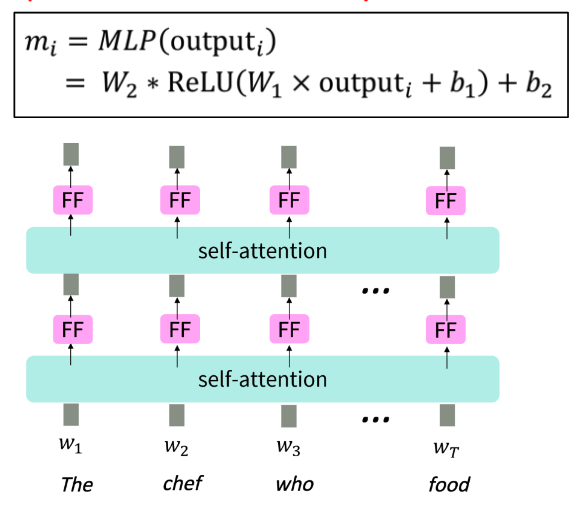
\includegraphics[scale=0.4]{img/stacked_self_attention_layers.png}
    \end{center}

    Boom, problem solved. 

    Going back, if we want to look at the attention for token $x_i$, we want to look through all $q_i^T k_j$ for all $j$ and find out where it is high. But perhaps we want to focus on different $j$ for different reasons. The following example may illustrate why. 

    \begin{example}[Semantic and Syntactic Attention]
      Given the sentence \textit{I went to the bank and got some money.}, one type of attention may look at the semantic meaning of the words, such as associating \textit{bank} with \textit{money}. However, we may also want to look at the syntactic meaning of the words, such as associating \textit{went} with \textit{bank}. When we read sentences, we have different types of attention for different reasons, and so having multiple heads of attention may be useful. 
    \end{example}

    \begin{definition}[Multi-Head Attention]
      Therefore, let us construct multiple attention heads by defining multiple triplets of $(Q, K, V)$ matrices. This may be more computationally inefficient, so we simply scale down the size of these matrices from 
      \[Q \in \mathbb{R}^{E_q \times d}, K \in \mathbb{R}^{E_k \times d}, V \in \mathbb{R}^{E_v \times d}\] 
      to 
      \[Q_\ell \in \mathbb{R}^{E_q \times d/h}, K_\ell \in \mathbb{R}^{E_k \times d/h}, V_\ell \in \mathbb{R}^{E_v \times d/h}\] 
      where $h$ is the number of heads. We are essentially decreasing the size of the token embedding dimension in order to get more heads. We can then do attention on each head separately. 
      \begin{equation} 
        \mathrm{Attention}_\ell = \mathrm{Attention}(Q_\ell, K_\ell, V_\ell) = \mathrm{softmax} \bigg( \frac{Q_\ell K_\ell^T}{\sqrt{E_k/h}} \bigg) V_\ell
      \end{equation}
      and we can simply concatenate them together to get the final output. 
      \[\mathrm{MultiHead}(Q, K, V) = \mathrm{Concat}(\mathrm{Attention}_1, \ldots, \mathrm{Attention}_h) W^O\]
      where $W^O \in \mathbb{R}^{d \times E_v}$ is a learnable weight matrix that mixes these heads together with a final linear transformation.\footnote{There is a valid concern that these heads may all end up learning the same thing and may just converge onto the same thing. However, this is not what happens in practice.} This entire process is shown in Figure \ref{fig:multi_head_attention}. 
    \end{definition}

    \begin{figure}[H]
      \centering 
      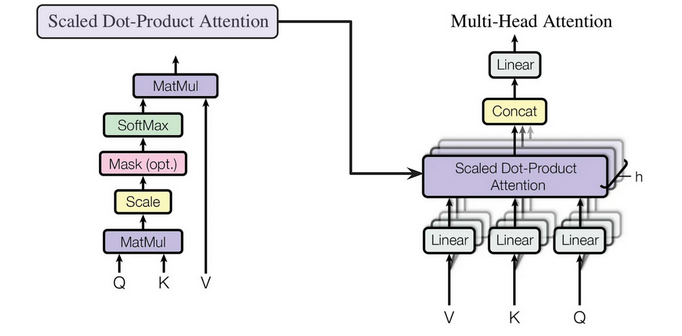
\includegraphics[scale=1.5]{img/multi_head_attention.png}
      \caption{Diagram of multi head attention. } 
      \label{fig:multi_head_attention}
    \end{figure}

\subsection{Transformers} 

    With self-attention out of the way, the transformer architecture becomes quite simple. An overview of it is shown in Figure \ref{fig:transformer}. 

    \begin{figure}[H]
      \centering 
      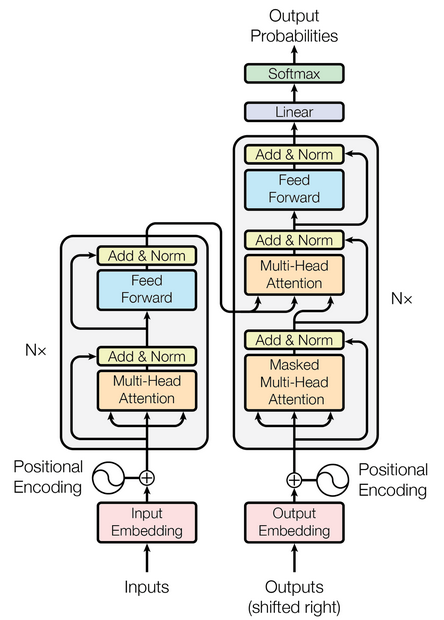
\includegraphics[scale=1.3]{img/transformer.png}
      \caption{Transformer architecture. } 
      \label{fig:transformer}
    \end{figure}

    The encoder is quite simple. You take the input embedding and add the positional embeddings to get $\{x_i \in \mathbb{R}^d\}_{i=1}^n$. You then pass it through a multi-head self-attention layer, which has outputs of shape $E_v \times n$, and then pass it through a feed forward network, adding residual connections and normalization layers to help with training. You then repeat this process $N$ times, which gives out the encoded sequence $\mathbf{h}_{1:n} = [\mathbf{h}_1, \ldots, \mathbf{h}_n]$, now ready to be fed into the decoder.\footnote{You can see that to support iterating through $n$ times, $E_v$ should equal $d$.}

    The decoder has two different self-attention layers. First, we run the generated output sequence through a masked self-attention layer, which generates the hidden nodes $\mathbf{z}_{1:n} = [\mathbf{z}_1, \ldots, \mathbf{z}_n]$ representing the state of the currently decoded sentence. Again, we have some maximum output length to ensure that we are working with a fixed size, and manually mask all tokens after the current one to be $0$.

    Then, another \textbf{cross-attention} layer takes both $\mathbf{h}_{1:n}$ and $\mathbf{z}_{1:n}$ and with its trained $(\mathbf{K}, \mathbf{V}, \mathbf{Q})$, computes the key, value, and query matrices as 
    \begin{equation}
      K = \mathbf{K} \mathbf{h}_{1:n}, \;\;\; V = \mathbf{V} \mathbf{h}_{1:n}, \;\;\; Q = \mathbf{Q} \mathbf{z}_{1:n}, 
    \end{equation}
    now ready to be plugged into to the self-attention formulas, integrating both the inputs and the current output to generate the result. This again outputs another list of vectors, which are run through an MLP and then have another set of $(\mathbf{K}, \mathbf{V}, \mathbf{Q})$ matrices waiting for them. This makes sense, since we want to use the output sequence to query the input key-values and attend to the correct set of tokens. 
    
    The output of this is then passed through a feed forward network, with some residual connections and normalization, and finally a linear layer transforms the output dimensions to whatever is needed (e.g. size of the vocabulary, or number of classes). Once this is done, a new word is generated,\footnote{Note that we have not specified how to get the corresponding word given an embedding vector. This is not within the scope of these notes and are covered in my natural language processing notes.} and this word (along with all previous words) is now used as the new input to the decoder in place of the start token. This process is done until the stop token is generated by the decoder. Notice that we encode with a bidirectional model (no masking) and generated the target with a unidirectional model (masking). 

    Note that again, parallelization of the decoder is not possible in the transformer architecture. Additionally, you can see that more normalization layers and residual connections are needed to train efficiently. This is very important in practice. 

    Despite all its advantages, self-attention has quadratic runtime complexity with respect to the sequence length since we need to compute attention for all pairs of words. This is worse than the linear runtime complexity in RNNs.  

  \subsubsection{Masking}

    The final aspect we did not address is the masking. When we are training the transformer on a corpus of data, the decoder first computes self-attention on all the previous outputs first to get the query, and then takes in the output of the encoder self-attention layer as the keys and values. Then it does self-attention once more over these triplets, essentially doing a self-attention layer over the entire input and all tokens up to the current decoded output. 

    When training this model, we have access to the entire decoded output, and we want to make sure that we do not perform self-attention on any future words since it will most likely attend 100\% to the next word to generate the next word! This does not learn anything, so we artificially set the attention distribution for all future output words to be $0$. This is usually done by setting the attention scores to $-\infty$ (or more practically, a very negative number) which will result in $0$ after softmaxing.\footnote{Here is a nice explanation \href{https://stackoverflow.com/questions/58127059/how-to-understand-masked-multi-head-attention-in-transformer}{here}.}

\subsection{Practical Implementation}

  In here we go over the nitty gritty details that comes into implementing a transformer in \texttt{pytorch==2.3.0}. 

  \subsubsection{Key, Value, Query Matrices and In Projections}

    The first thing is that these key, value, query does not have to necessarily equal to the dimension embedding, which we will denote as $E$. One flexibility is that we don't necessarily need to set the dimensions of the keys, values, and queries the same. We can see in the constructor of the \texttt{torch.nn.MultiheadAttention} module that you can input your own dimensions for the keys and values, but queries must be the same as $E$. 
    \begin{lstlisting}
      def __init__(self, embed_dim, num_heads, dropout=0., bias=True, add_bias_kv=False, add_zero_attn=False,
                   kdim=None, vdim=None, batch_first=False, device=None, dtype=None) -> None:
         ... 
        self.embed_dim = embed_dim
        self.kdim = kdim if kdim is not None else embed_dim
        self.vdim = vdim if vdim is not None else embed_dim
        self._qkv_same_embed_dim = self.kdim == embed_dim and self.vdim == embed_dim
    \end{lstlisting}

    In fact, $K \in \mathbb{R}^{d_k \times E}$, $V \in \mathbb{R}^{d_v \times E}$, then $QK^T \in \mathbb{R}^{E \times d_k}$. Since this obviously leads to dimension mismatch problem when we multiply it with the matrix $V$, what we do is have an \textbf{in projection} layer that maps everything to dimension $E$. We can check this for the following. 
    \begin{equation}
      K_{proj} \in \mathbb{R}^{E \times d_k}, V_{proj} \in \mathbb{R}^{E \times d_v}, Q_{proj} \in \mathbb{R}^{E \times E}
    \end{equation}
    There are two ways to store these projection matrices, as shown in the constructor. 
    \begin{lstlisting}
      # in the constructor 
      ...
      self._qkv_same_embed_dim = self.kdim == embed_dim and self.vdim == embed_dim

      if not self._qkv_same_embed_dim:
        self.q_proj_weight = Parameter(torch.empty((embed_dim, embed_dim), **factory_kwargs))
        self.k_proj_weight = Parameter(torch.empty((embed_dim, self.kdim), **factory_kwargs))
        self.v_proj_weight = Parameter(torch.empty((embed_dim, self.vdim), **factory_kwargs))
        self.register_parameter('in_proj_weight', None)
      else:
        self.in_proj_weight = Parameter(torch.empty((3 * embed_dim, embed_dim), **factory_kwargs))
        self.register_parameter('q_proj_weight', None)
        self.register_parameter('k_proj_weight', None)
        self.register_parameter('v_proj_weight', None)
    \end{lstlisting}
    \begin{enumerate}
      \item If these shapes are different, then we store them in separate matrices as above. 
      \begin{lstlisting}
        att = nn.MultiheadAttention(embed_dim=50, num_heads=1, bias=False, kdim=30, vdim=40) 
        att.q_proj_weight.shape # torch.Size([50, 50])
        att.k_proj_weight.shape # torch.Size([50, 30])
        att.v_proj_weight.shape # torch.Size([50, 40])
      \end{lstlisting}

      \item If these shapes are the same, then we just store them in a $3E \times E$ matrix by concatenation them. 
      \begin{lstlisting}
        att = nn.MultiheadAttention(embed_dim=50, num_heads=1, bias=False) 
        att.in_proj_weight.shape # torch.Size([150, 50])
      \end{lstlisting}
    \end{enumerate}
    These conditions are asserted throughout the forward pass as well.  

  \subsubsection{Masking} 

    We multiply by a masking matrix. 

  \subsubsection{Computing Attention}

    First we reshape them so that they are batch first. 

    If \texttt{needs\_weights = True}, we also output the attention weights in addition to the output, but it is said that this degrades performance. It is by default true but should be set to false for small tasks. 

  \subsubsection{Forward Pass of MultiheadAttention}

    First, we should look at the main function that computes self-attention. We omit a large part of the code to focus on the relevant details. 

    \begin{lstlisting}
      # torch.nn.functional 
      def multi_head_attention_forward(
        query: Tensor,
        key: Tensor,
        value: Tensor,
        embed_dim_to_check: int,
        num_heads: int,
        in_proj_weight: Optional[Tensor],
        in_proj_bias: Optional[Tensor],
        bias_k: Optional[Tensor],
        bias_v: Optional[Tensor],
        add_zero_attn: bool,
        dropout_p: float,
        out_proj_weight: Tensor,
        out_proj_bias: Optional[Tensor],
        training: bool = True,
        ...
      ): 
      # first unsqueezes the input if it is not batched. 

      # look at the input dimensions and check that multiheads divide it evenly 
      #  
      assert embed_dim == embed_dim_to_check, \
          f"was expecting embedding dimension of {embed_dim_to_check}, but got {embed_dim}"
      if isinstance(embed_dim, torch.Tensor):
          # embed_dim can be a tensor when JIT tracing
          head_dim = embed_dim.div(num_heads, rounding_mode='trunc')
      else:
          head_dim = embed_dim // num_heads
      assert head_dim * num_heads == embed_dim, f"embed_dim {embed_dim} not divisible by num_heads {num_heads}"
      if use_separate_proj_weight:
          # allow MHA to have different embedding dimensions when separate projection weights are used
          assert key.shape[:2] == value.shape[:2], \
              f"key's sequence and batch dims {key.shape[:2]} do not match value's {value.shape[:2]}"
      else:
          assert key.shape == value.shape, f"key shape {key.shape} does not match value shape {value.shape}"

      # Computes in-projection, which is an affine map before doing attention. 
      # in_proj_weight = [W_q, W_k, W_v], in_proj_bias = [b_q, b_k, b_v] 
      # computes q = q * W_q + b_q, k = k * W_k + b_k, v = v * W_v + b_v
      if not use_separate_proj_weight:
        q, k, v = _in_projection_packed(query, key, value, in_proj_weight, in_proj_bias)
      else:
        if in_proj_bias is None:
            b_q = b_k = b_v = None
        else:
            b_q, b_k, b_v = in_proj_bias.chunk(3)
        q, k, v = _in_projection(query, key, value, q_proj_weight, k_proj_weight, v_proj_weight, b_q, b_k, b_v)

      # prepare attention mask 
      # add bias along batch dimension  
      # more preparation with mask
      ... 
      # Now calculate attention
      if need_weights:
        # scale q_scale for the sqrt(E) division factor 
        B, Nt, E = q.shape
        q_scaled = q * math.sqrt(1.0 / float(E))

      if attn_mask is not None:
        # torch.baddbmm is a pybinded C function implementing matrix multiplication 
        # of form attn_mask + q_scaled @ k^T
        attn_output_weights = torch.baddbmm(attn_mask, q_scaled, k.transpose(-2, -1))
      else:
        # torch.bmm is also a pybinded C function q_scaled + k^T
        attn_output_weights = torch.bmm(q_scaled, k.transpose(-2, -1))
      ...
      # softmax it and then multiply it by V. 
      attn_output_weights = softmax(attn_output_weights, dim=-1)
      attn_output = torch.bmm(attn_output_weights, v)

      # final linear layer for more weightings. 
      attn_output = attn_output.transpose(0, 1).contiguous().view(tgt_len * bsz, embed_dim)
      attn_output = linear(attn_output, out_proj_weight, out_proj_bias)
      attn_output = attn_output.view(tgt_len, bsz, attn_output.size(1))

      # optionally average attention weights over heads
      attn_output_weights = attn_output_weights.view(bsz, num_heads, tgt_len, src_len)
      if average_attn_weights:
          attn_output_weights = attn_output_weights.mean(dim=1)

      if not is_batched:
          # squeeze the output if input was unbatched
          attn_output = attn_output.squeeze(1)
          attn_output_weights = attn_output_weights.squeeze(0)
      return attn_output, attn_output_weights
    \end{lstlisting}

    This is precisely the function that is called in the forward method of the \texttt{MultiheadAttention} module. 

  \subsubsection{Transformer}

    In the transformer, we can see that if we peek at the state dictionary, it composes of an encoder and a decoder, each with a certain number of attention layers. There are 6 attention layers each by default. 

    \begin{lstlisting}
      transformer = nn.Transformer()
      transformer.state_dict
      # output 
      <bound method Module.state_dict of Transformer(
        (encoder): TransformerEncoder(
          (layers): ModuleList(
            (0-5): 6 x TransformerEncoderLayer(
              (self_attn): MultiheadAttention(
                (out_proj): NonDynamicallyQuantizableLinear(in_feat
      ures=512, out_features=512, bias=True)
              )
              (linear1): Linear(in_features=512, out_features=2048,
       bias=True)
              (dropout): Dropout(p=0.1, inplace=False)
              (linear2): Linear(in_features=2048, out_features=512,
       bias=True)
              (norm1): LayerNorm((512,), eps=1e-05, elementwise_aff
      ine=True)
              (norm2): LayerNorm((512,), eps=1e-05, elementwise_aff
      ine=True)
              (dropout1): Dropout(p=0.1, inplace=False)
              (dropout2): Dropout(p=0.1, inplace=False)
            )
          )
          (norm): LayerNorm((512,), eps=1e-05, elementwise_affine=T
      rue)
        )
        (decoder): TransformerDecoder(
          (layers): ModuleList(
            (0-5): 6 x TransformerDecoderLayer(
              (self_attn): MultiheadAttention(
                (out_proj): NonDynamicallyQuantizableLinear(in_feat
      ures=512, out_features=512, bias=True)
              )
              (multihead_attn): MultiheadAttention(
                (out_proj): NonDynamicallyQuantizableLinear(in_feat
      ures=512, out_features=512, bias=True)
              )
              (linear1): Linear(in_features=512, out_features=2048,
       bias=True)
              (dropout): Dropout(p=0.1, inplace=False)
              (linear2): Linear(in_features=2048, out_features=512,
       bias=True)
              (norm1): LayerNorm((512,), eps=1e-05, elementwise_aff
      ine=True)
              (norm2): LayerNorm((512,), eps=1e-05, elementwise_aff
      ine=True)
              (norm3): LayerNorm((512,), eps=1e-05, elementwise_aff
      ine=True)
              (dropout1): Dropout(p=0.1, inplace=False)
              (dropout2): Dropout(p=0.1, inplace=False)
              (dropout3): Dropout(p=0.1, inplace=False)
            )
          )
          (norm): LayerNorm((512,), eps=1e-05, elementwise_affine=T
      rue)
        )
      )>
    \end{lstlisting}

\subsection{Vision Transformers} 

  We have hinted at attention being applicable in other architectures, and the most popular is in computer vision. Historically, CNNs were very useful because they take into account the locality and translational-invariance of objects in images inherently in the convolutions. This is a great strength of convolutional networks. 
  
  Can transformers beat this? These assumptions are not built into the architecture, and researchers were quite unsuccessful in passing the benchmarks set by CNNs, but it turned out that in 2020, with enough training and a large enough architecture, \textit{vision transformers} in fact did surpass CNNs. 


\bibliographystyle{alpha}
\bibliography{./bibfile}
\end{document}

